\chapter{Covers}
\label{chapter:covers}

The COATLI telescope was originally equipped with M1 covers supplied by ASTELCO and controller by a PLC in a cabinet in the shed. These were removed in October 2017 to reduce wind shake. The cabinet is still installed (as it also contains the secondary controller) and the covers are stored in the COATLI/DDOTI warehouse. This appendix remains as a historic reference.

\section{Description}

\begin{figure*}
\begin{center}
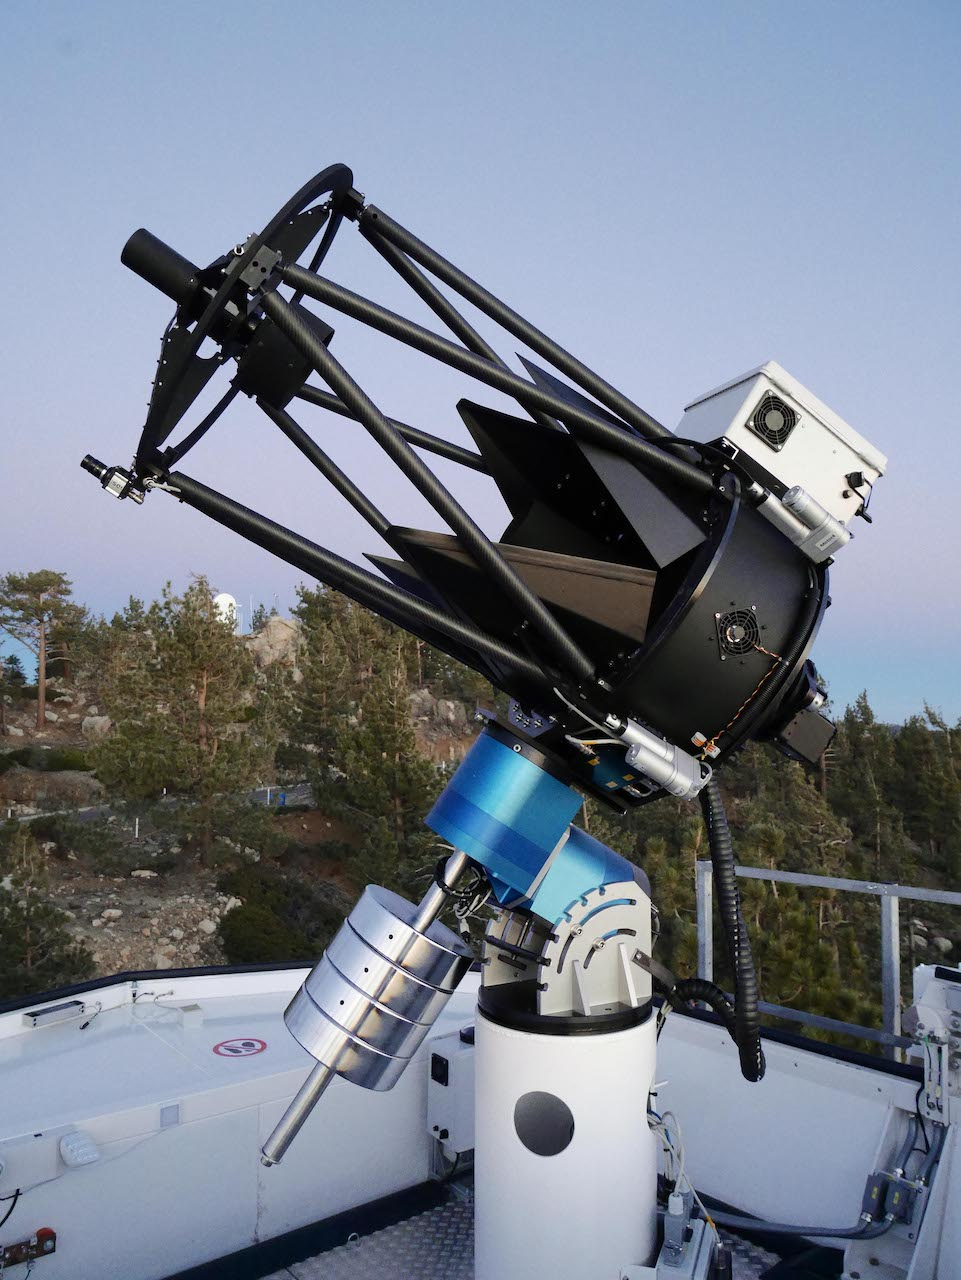
\includegraphics[width=0.8\linewidth]{figures/covers-open.jpg}
\end{center}
\caption{The covers that protect the telescope and instrument, here shown open.}
\label{figure:covers-open}
\end{figure*}

\begin{figure*}
\begin{center}
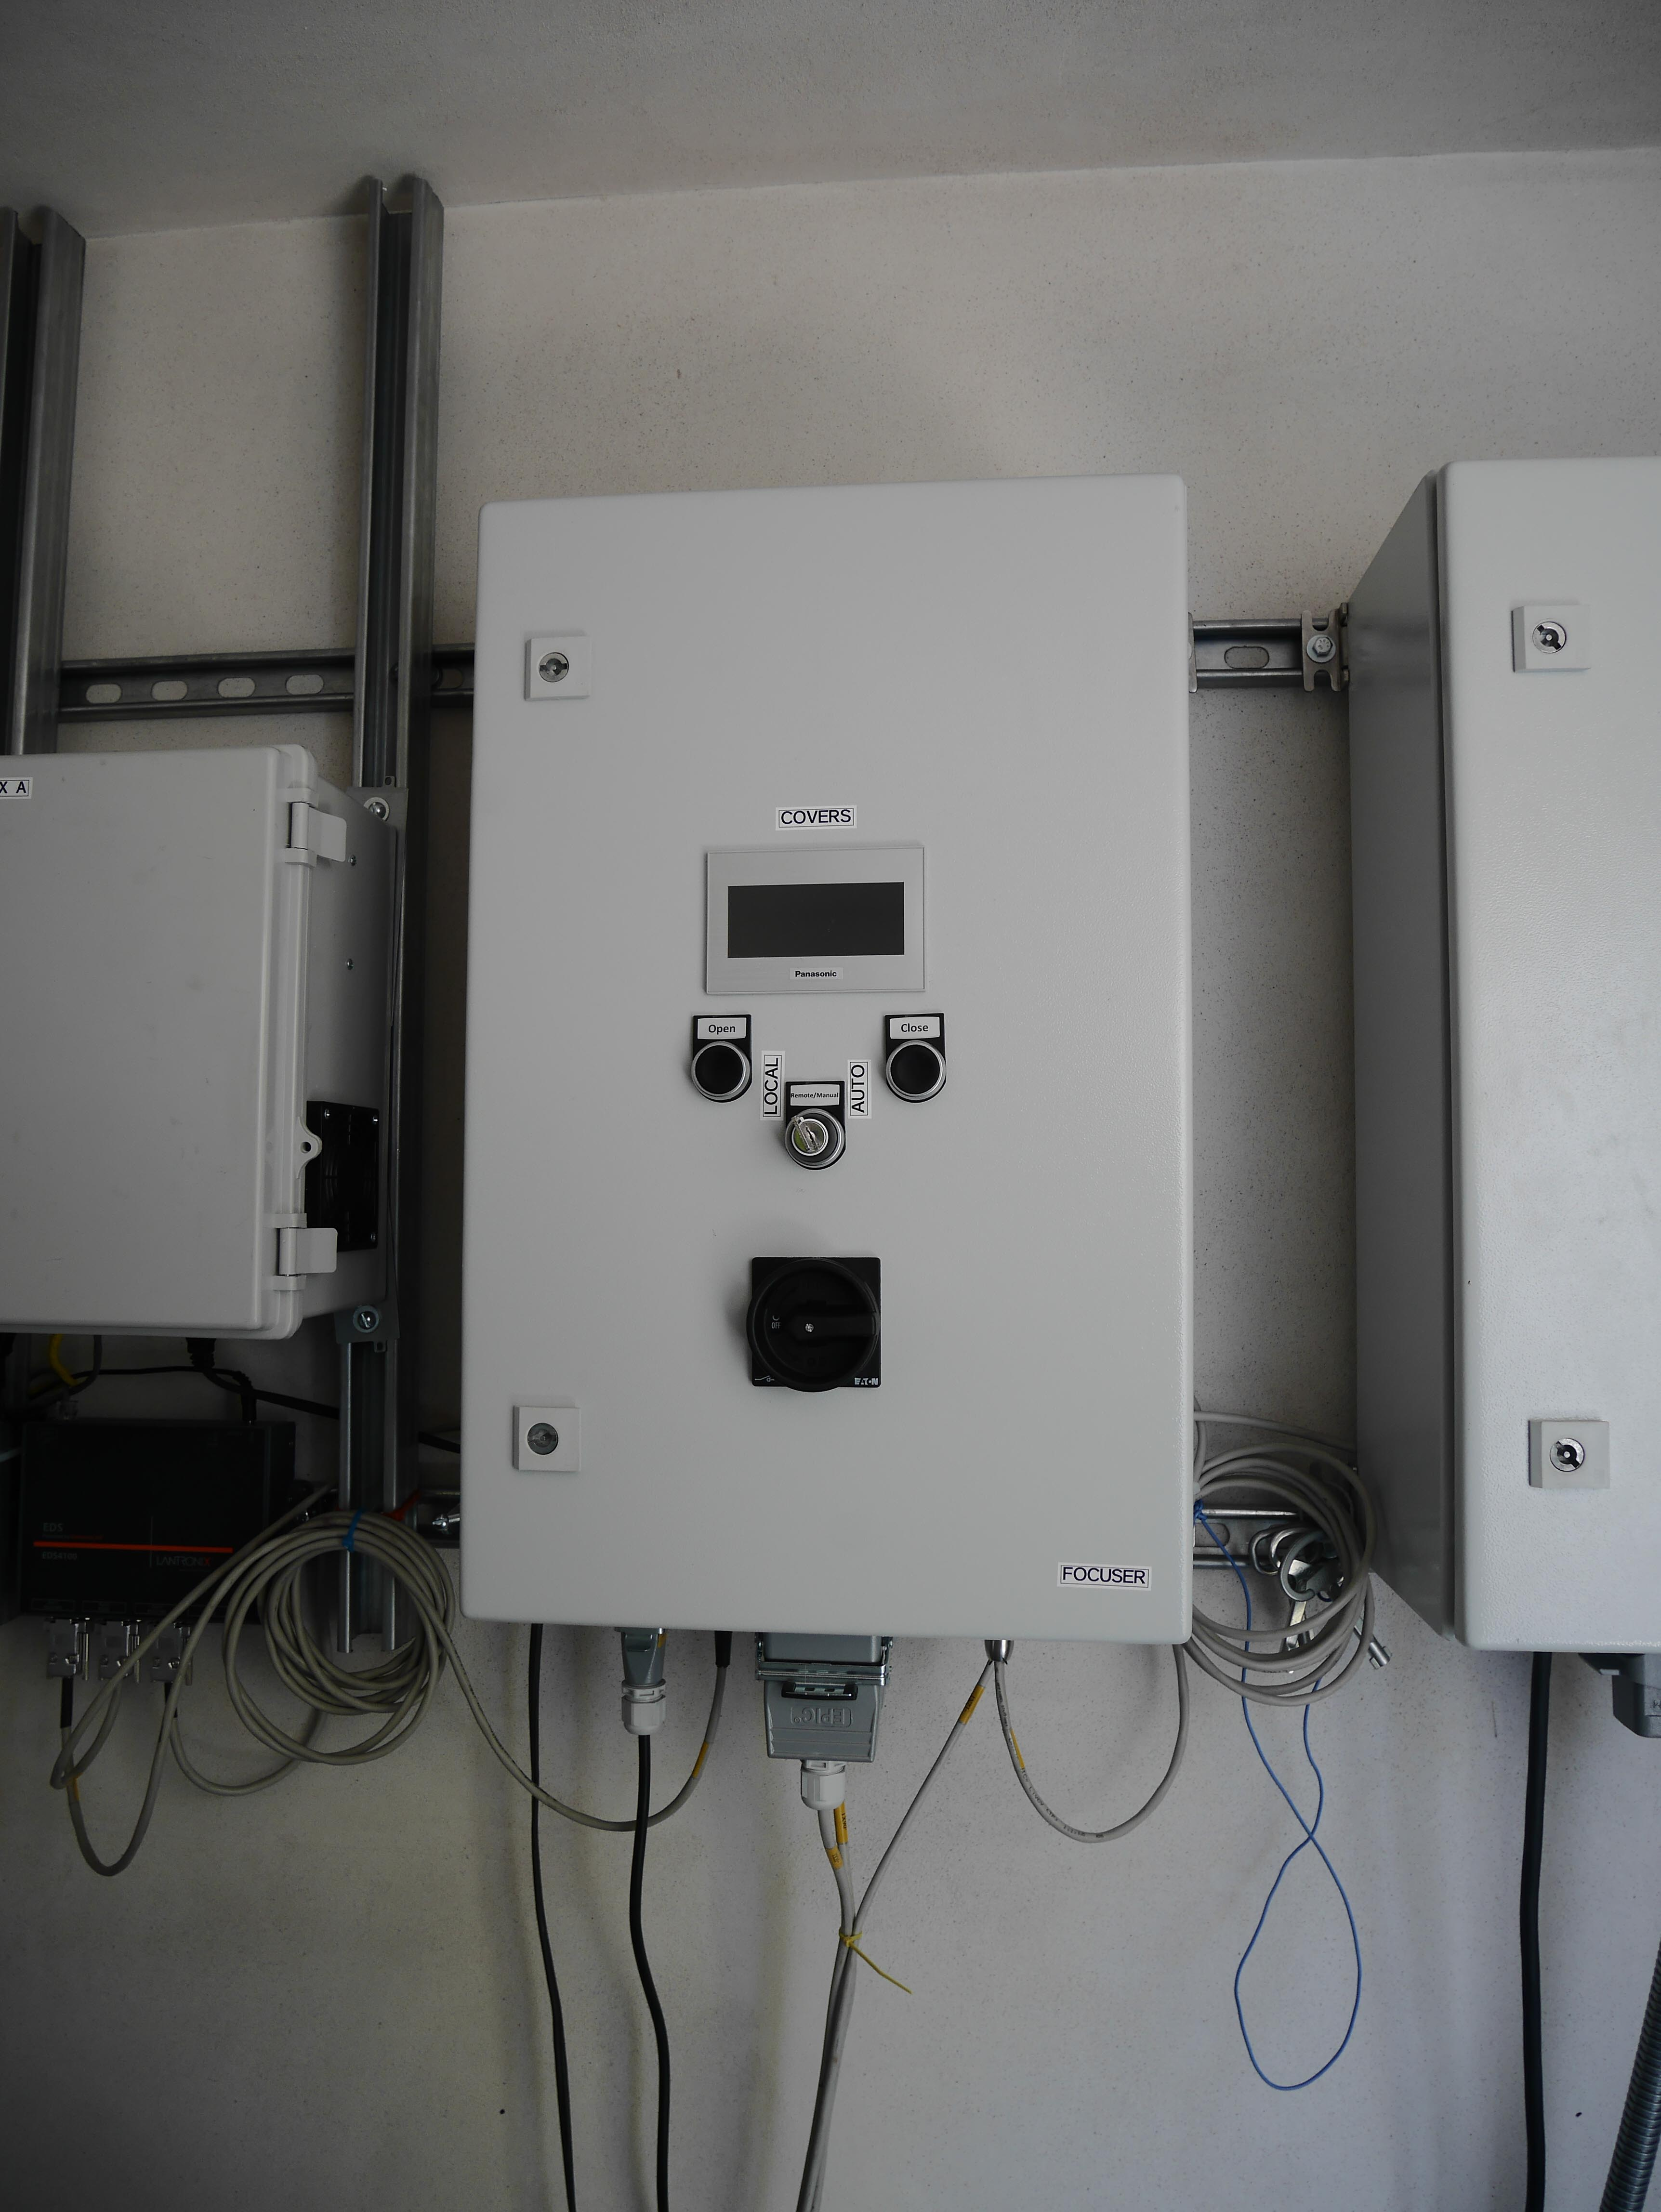
\includegraphics[width=0.8\linewidth]{figures/covers-controller.jpg}
\end{center}
\caption{The covers controller in the shed, between Box A (left) and the covers controller (right).}
\label{figure:covers-controller}
\end{figure*}

\begin{figure*}
\begin{center}
\resizebox{\linewidth}{!}{\begin{labeled}{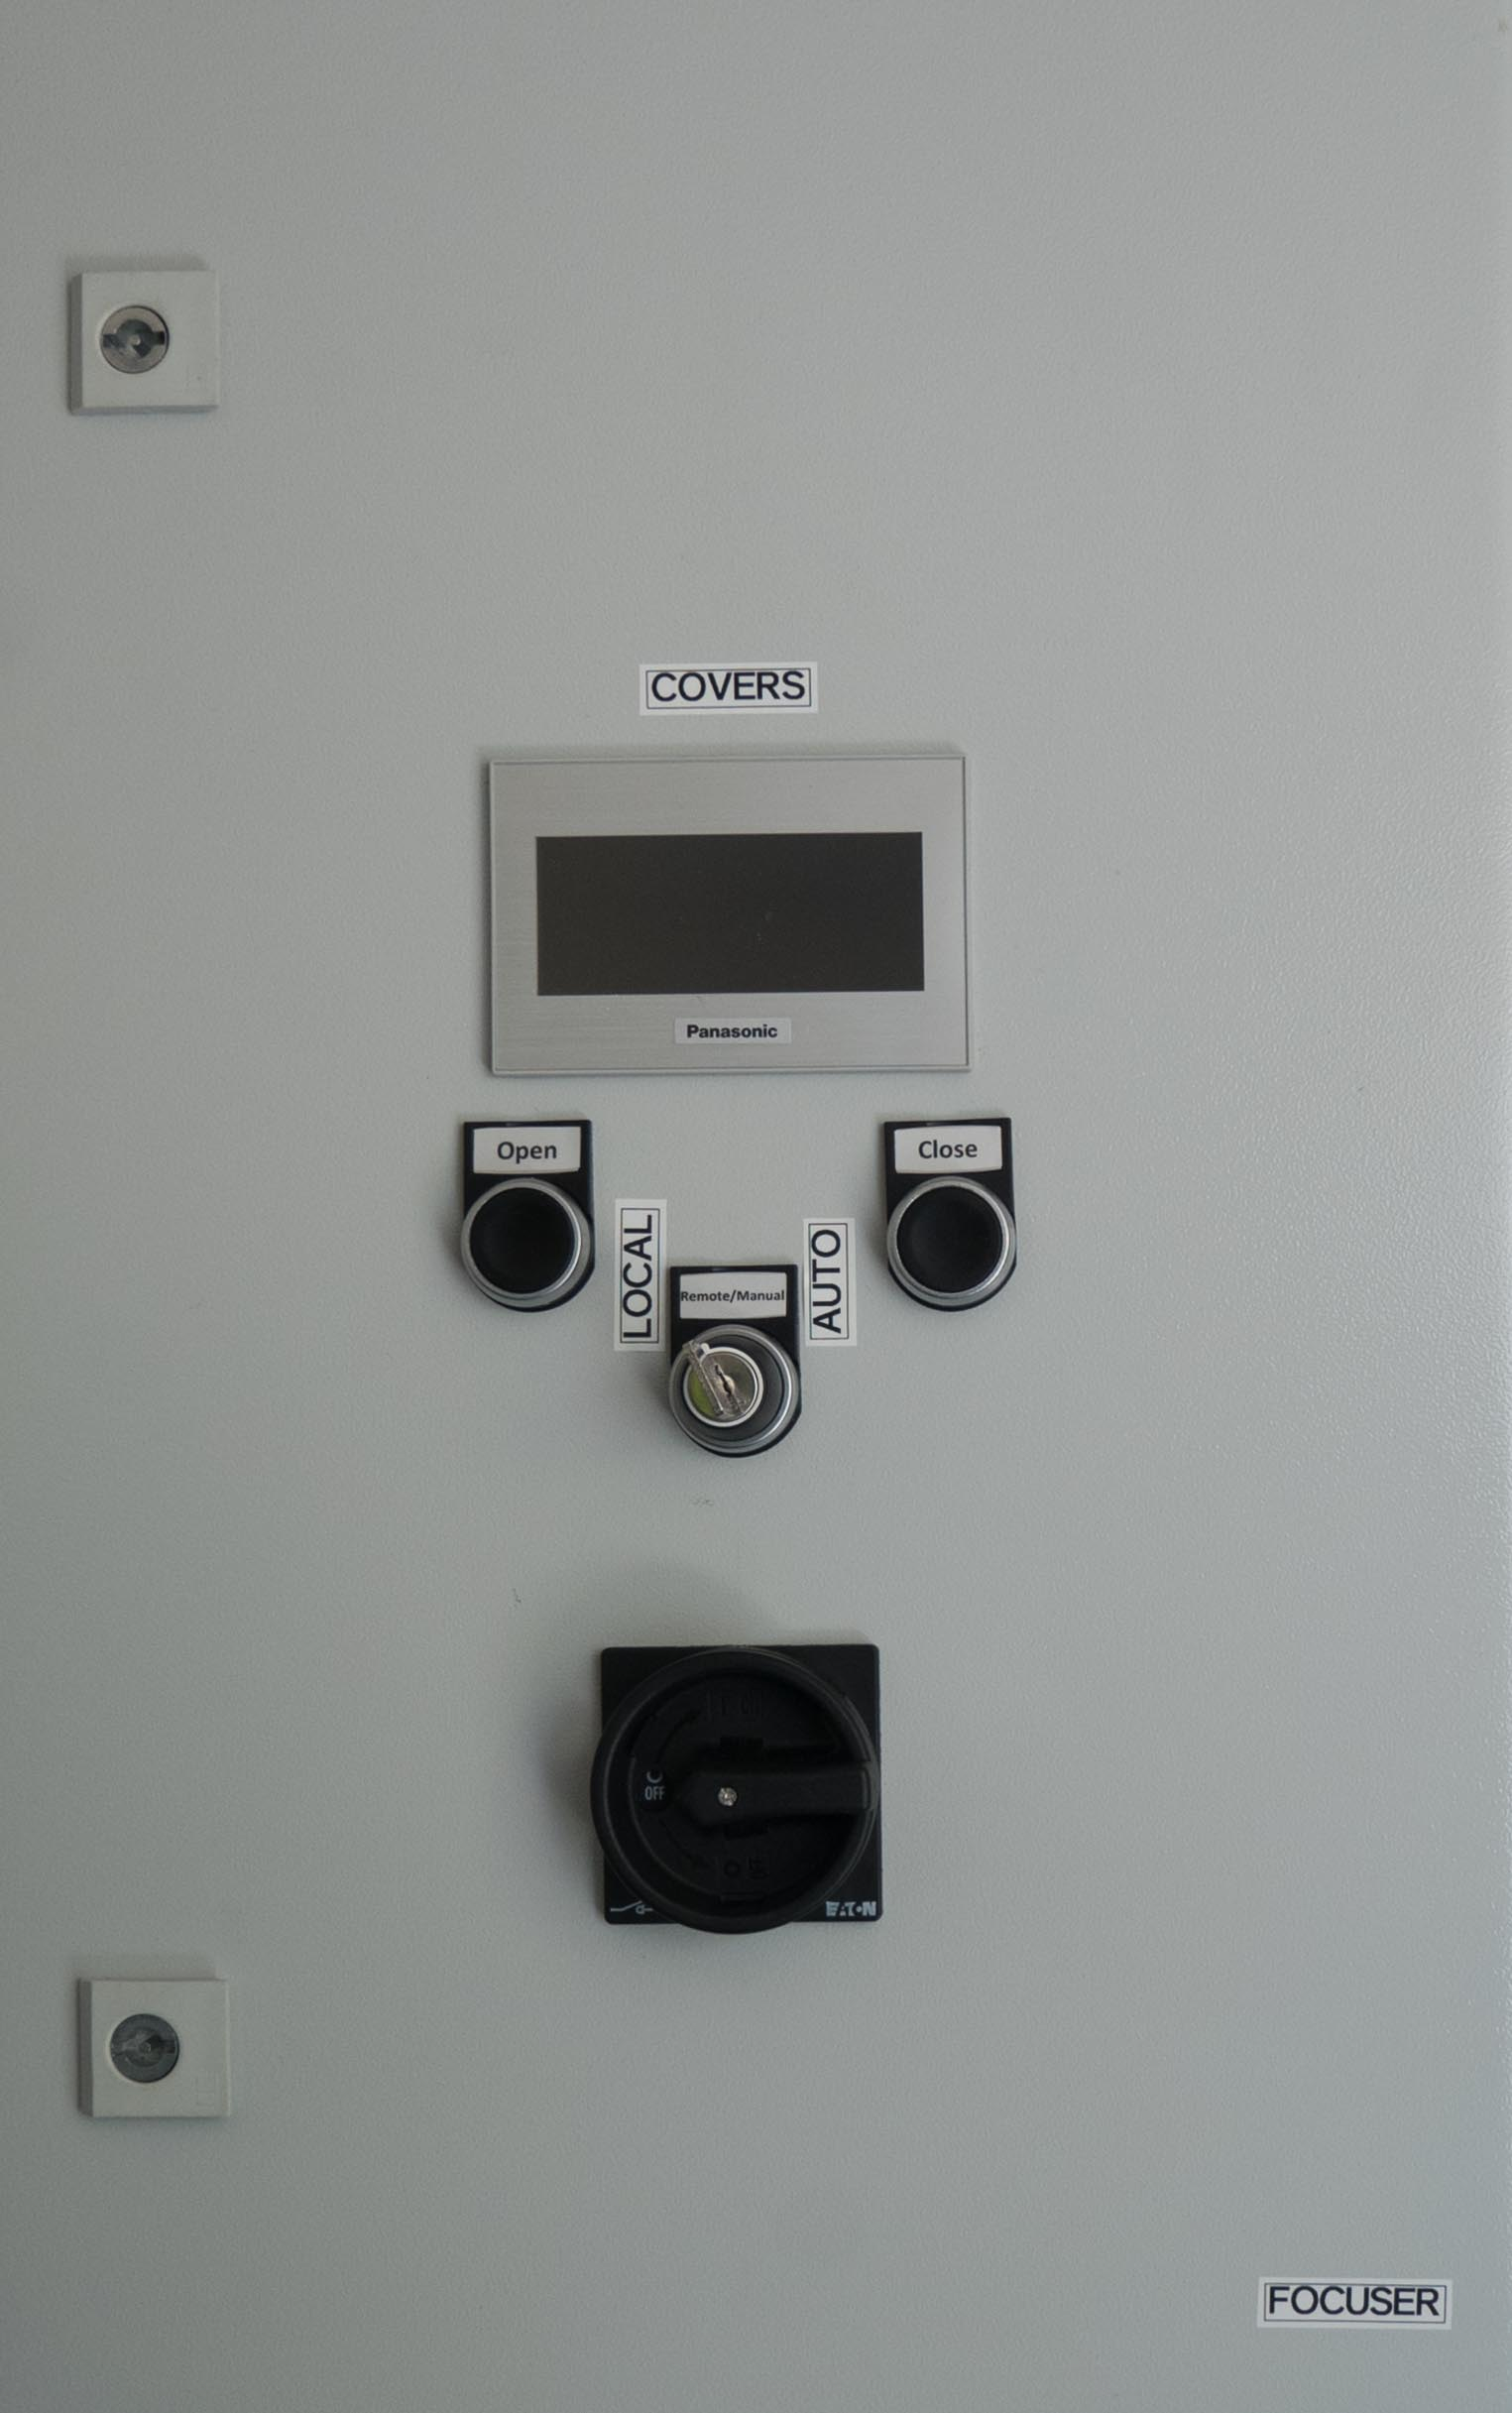
\includegraphics[width=0.5\linewidth]{figures/covers-controller-door.jpg}}
%\draw[dotted] (-5,-5) grid (+5,+5);
\arrowandlabel{(-0.3,-1.0)}{(-3.0,-5.4)}{north}{Mode Selector Switch};
\arrowandlabel{(0.5,-3)}{(+3.0,-5.4)}{north}{Main Power Switch};
\arrowandlabel{(-1.2,+0.2)}{(-3.0,+5.4)}{south}{Open Button};
\arrowandlabel{(+1.1,+0.2)}{(+3.0,+5.4)}{south}{Close Button};
\arrowandlabel{(+0.0,+1.5)}{(+0.0,+5.4)}{south}{LCD Display};
\end{labeled}}
\end{center}
\caption{The covers controller door and control panel. Bottom: the main power switch. Middle, left to right: the open button, the mode selector switch (“LOCAL” and “REMOTE”), and the close button. Top: the LCD display.}
\label{figure:covers-controller-door}
\end{figure*}

The COATLI telescope is protected by covers, supplied by ASTELCO, which close to seal the space over the primary mirror and the primary baffle. These are shown in Figure~\ref{figure:covers-open}. The covers are divided into four petals, which open and close in oposite pairs. The covers are opened by Transmotec DLA-24-40-A-50-IP65-NC linear actuators.

The covers can be controller locally or remotely.

The controller for the covers, shown in Figure~\ref{figure:covers-controller} is located in a cabinet in the shed. The controller is powered by 220 V 60 Hz from Circuit A via the 220 V UPS and 220 V iBootBar. The covers controller cabinet also houses the focuser controller for the secondary.

\safety{The covers should normally be closed while opening or closing the covers, to protect the telescope and instrument.}

The covers controller can be in local or remote mode. The mode is selected by the switch on the door of the covers controller in the shed (see Figure~\ref{figure:covers-controller-door}). In remote mode

\begin{enumerate}
\item
The switches on the covers controller to open and close the covers are deactivated.
\item
The robotic control system can open and close.
\end{enumerate}

In local mode:

\begin{enumerate}
\item
The switches on the covers controller to open and close the covers are active.
\item
The robotic control system cannot open and close.
\end{enumerate}

\section{Maintenance Procedures}

\subsection{Enabling Remote Mode}

\subsubsection{Safety Considerations}

\safety{In local mode, the control system can open or close the covers.}

\subsubsection{Requirements}

You will need:
\begin{itemize}
\item One person.
\item The key to the shed (see \S\ref{section:shed-key}).
\end{itemize}

\subsubsection{Procedure}

\begin{enumerate}
\item
Go to the shed.
\item
Move the main power switch on the covers controller to “ON”.
\item
Move the mode selector switch on the covers controller door to “REMOTE”.
\end{enumerate}


\subsection{Opening or Closing in Local Mode}
\label{section:covers-opening-or-closing-in-local-mode}

\subsubsection{Safety Considerations}

\safety{In local mode, the control system cannot open or close the covers.}

\safety{Before opening the covers, check on the webcams that the covers is not open and the telescope is not pointed to towards the sun. In the home position, the telescope is pointed to the north pole.}

\subsubsection{Requirements}

You will need:

\begin{itemize}
\item One person.
\item The key to the shed (see \S\ref{section:shed-key}).
\end{itemize}

\subsubsection{Procedure}

\begin{enumerate}
\item
Go to the shed.
\item
Move the main power switch on the covers controller door to “ON”.
\item
Move the mode selector switch on the covers controller door to “LOCAL”.
\item
To open, press and hold the open button until the LCD display indicates that the covers are open.
\item
To close, press and hold the close button until the LCD display indicates that the covers are closed.
\item
If you wish to subsequently operate the covers remotely, move the mode selector switch to “REMOTE”.
\end{enumerate}

\section{Remote Interface}
\label{section:covers-remote-interface}

\subsection{Lantronix EDS}
\label{section:covers-lantronix-eds}

The RS-232 interface to the covers controller is made available via the Lantronix EDS 4100 ethernet-to-serial converter. Specifically, it is connected to line 1 and configured 9600/8-N-1 with a tunnel on TCP port 10001.

The Lantronix EDS is on the LAN at \verb|lantronix-eds|.

\subsection{ADAM Modules}
\label{section:covers-adam-modules}

Remote control of the covers is through an ADAM-4055 digital input/output module. The input and output channels of the ADAM-4055 module are connected to the covers controller PLC.

The RS-485 serial interface of the ADAM-4055 is exposed via an ADAM-4520 RS-232 to RS-485 converter and isolator as RS-232 at 9600/8-N-1.

The state of the input and output channels can be determined either from the web interface (the “Input Channels” and “Output Channels” variables in the “covers” tab) or by unscrewing the ADAM-4520 RS-232 to RS-485 converter on top of the ADAM-4055 to reveal LEDs which show the state of the channels.

The input channels are:
\begin{description}
\item[DI0] Open. 0 = not open and 1 = open. This channel is connected to terminal Y8 on the PLC via relay 8K1.
\item[DI1] Closed. 0 = not closed and 1 = closed. This channel is connected to terminal Y9 on the PLC via relay 8K2.
\item[DI2] Reserved. This channel is connected to terminal YA on the PLC via relay 8K3.
\item[DI3] Mode. 0 = local and 1 = remote. This channel is connected to terminal Yb on the PLC via relay 8K4. 
\item[DI4] Not used.
\item[DI5] Not used.
\item[DI6] Not used.
\item[DI7] Not used.
\end{description}

The output channels are:
\begin{description}
\item[DO0] Open or close selector. Set to 0 to select open and 1 to select close. Setting this bit does not initiate the movement.
This channel is connected to terminal X4 of the PLC.
\item[DO1] Move. Set to 1 to carry out the movement specified by DO0. This channel is connected to terminal X5 of the PLC.
\item[DO2] Reserved. This channel is connected to terminal X6 on the PLC.
\item[DO3] Reserved. This channel is connected to terminal X7 on the PLC.
\item[DO4] Not used.
\item[DO5] Not used.
\item[DO6] Not used.
\item[DO7] Not used.
\end{description}

\subsection{Diagnostics}

To check communication with the Lantronix EDS, from a terminal run:

\begin{quotation}
\begin{verbatim}
ping lantronix-eds
\end{verbatim}
\end{quotation}

To check communication with the ADAM modules, from a terminal on \verb|control|, first stop the covers server so that it releases the covers TCP port on the Lantronix EDS:

\begin{quotation}
\begin{verbatim}
sudo stopserver covers
\end{verbatim}
\end{quotation}

Then connect to the covers TCP port on the Lantronix EDS using telnet:

\begin{quotation}
\begin{verbatim}
telnet lantronix-eds 10001
\end{verbatim}
\end{quotation}

You can then send commands to the ADAM-4055. Some useful commands (which should be followed by ENTER) are:

\begin{itemize}
\item Command: \verb|$01M|

Response: \verb|!014055|

Read Module Name. The response shown above confirms that you are talking to an ADAM-4055.

\item 
Command: \verb|$016|

Response: \verb|!|$XXYY$\verb|00|

Digital Data In. The values of the output channels (in upper-case hexadecimal) are given by $XX$ and the values of the input channels (in upper-case hexadecimal) are given by $YY$.

\item 
Command: \verb|#0100|$XX$

Response: \verb|>|

Digital Data Out. The output channels are set to $XX$ (in upper-case hexadecimal).

\end{itemize}

For more details of the commands, see the ADAM-4000 Manual.

You can exit from telnet by typing CTRL-\verb|]| and then \verb|quit|. Once you have done so, you should probably restart the covers server on \verb|control| with:

\begin{quotation}
\begin{verbatim}
sudo startserver covers
\end{verbatim}
\end{quotation}

\section{Control}

The server for the covers runs on \verb|control|. 

The server starts automatically when \verb|control| is rebooted, but if necessary can be stopped, started, or restarted explicitly by issuing the following commands on \verb|control|:
\begin{itemize}
\item
\verb|sudo stopserver covers|
\item
\verb|sudo startserver covers|
\item
\verb|sudo restartserver covers|
\end{itemize}

Server requests can be issued from any of the Mac or Linux machines on the COATLI LAN. The following requests are supported:

\begin{itemize}
\item
\verb|request covers initialize|

Initialize the server and covers hardware. As part of the process of initializing, the covers will close.

For this request to be accepted, the server activity must not be \verb|starting| or \verb|error|.

If the request is accepted, the server activity changes to \verb|initializing| and then, once it has initialized, to \verb|idle|.

\item
\verb|request covers open|

Open the covers.

For this request to be accepted, the server activity must not be \verb|starting|, \verb|started|, \verb|initializing|, or \verb|error|.

If the request is accepted, the server activity changes to \verb|opening| and then, once it has opened, to \verb|idle|.

\item
\verb|request covers close|

Close the covers.

For this request to be accepted, the server activity must not be \verb|starting|, \verb|started|, \verb|initializing|, or \verb|error|.

If the request is accepted, the server activity changes to \verb|closing| and then, once it has closed, to \verb|idle|.

\item
\verb|request covers stop|

Stop the covers.

For this request to be accepted, the server activity must not be \verb|starting| or \verb|error|.

If the request is accepted, the server activity changes to \verb|stopping| and then, once it has stopped, to \verb|started| (if the server has not been initialized) or to the activity after the previous completed request.

\item
\verb|request covers reset|

Reset an error in the covers.

\item
\verb|request covers status|

Show the status of the server.

Obtain the values of the status data from the server and print them to stdout.
\end{itemize}

\section{Bibliography}

\begin{flushleft}
\begin{itemize}
\item \href{bibliography/astelco-covers-electronics-schematic.pdf}{Electronic Schematics}, ASTELCO, Version 1.1.
\item “\href{bibliography/lantronix-eds-user-guide.pdf}{Lantronix EDS Device Servers/Terminal Servers User Guide}”, Lantronix, Revision 1 April 2011.
\item “\href{bibliography/advantech-adam-4000.pdf}{ADAM-4000 Data Adquisition Modules User's Guide]}”, Advantech, Edition 10.5, 2007.
\item “\href{bibliography/transmotec-dla.pdf}{Transmotec DLA Series Linear Actuators (2017).}
\end{itemize}
\end{flushleft}


